% !TeX encoding = UTF-8 Unicode
% !TeX root = manual.tex
% !TeX spellcheck = en_GB

\chapter{Code to produce the images and results from~\cite{Mej20}}

All figures are printed with Matlab. In order to reproduce them, additionally the 
\verb|export_fig| package, available at \href{https://de.mathworks.com/matlabcentral/fileexchange/23629-export_fig}%
{\emph{mathworks.com/matlabcentral/fileexchange/23629}} 
is necessary.
Furthermore, the following anonymous functions are used.

{\small%
\begin{lstlisting}
clc;
warning('off','MATLAB:MKDIR:DirectoryExists');
warning('off','MATLAB:LargeImage');

DPI='-r600';        %resolution
EXT='-pdf';         %default file format
BASE='.';           %base folder
AA='-a1';           %anti-aliasing. a1=off, a3=a lot
LGREY=[.6 .6 .6];   %color for light-grey
DGREY=[.4 .4 .4];
BLACK=[0 0 0];      %color for black
DOTSIZE=4;          %size of markers and dots
LINESIZE=.5;        %width of lines
FONTSIZE=8;         %font size

% %%%%%%%%%%%%%%%%%%%%%%%%
set(groot,'defaultAxesTickLabelInterpreter','latex');  
set(groot,'defaulttextinterpreter','latex');
set(groot,'defaultLegendInterpreter','latex');

FIGURE = @() figure('Units','Centimeters','Position',[0 0 25 25]);
TITLE = @(T) title(T,'Interpreter','latex');
AXISE = @(A) eval('axis(''equal''); axis(A)');
AXIS = @(A) eval('axis(A)');
LABEL = @(X,Y) eval(['xlabel(X,''Interpreter'',''Latex'');'...
   'ylabel(Y,''Interpreter'',''Latex'');']);
TICKS = @(X,Y) eval('xticks(X); yticks(Y);');
TICKLABELS = @(X,Y) eval('xticklabels(X); yticklabels(Y);');
SIZE = @(X,Y) set(gca,'Units','Centimeters','Position',[3 3 3*X 3*Y]);
SIZE1 = @() set(gca,'Units','Centimeters','Position',[3 3 15 1]);
TEXT = @(X,Y,T) text(X, Y, T,'Interpreter','Latex','Fontsize',FONTSIZE);
POST = @() eval(['set(findall(gcf,''-property'',''FontSize''),''FontSize'',' ...
   num2str(FONTSIZE) ' );'...
   'set(gca,''TickLabelInterpreter'', ''Latex'');'...
   'set(gcf, ''Color'', ''w'');'...
   'set(gca,''XMinorTick'',''off'',''YMinorTick'',''off'');'...
   'box on']);    
SAVE = @(FOLDER,NAME,EXT) eval(['mkdir(fullfile('''',''' BASE ''', FOLDER));'...
   'export_fig(fullfile('''', ''' BASE ''',FOLDER,NAME), ''-grey'', ''' DPI ...
   ''', ''' AA ''', ''' EXT ''', ''-dCompatibilityLevel=1.4'');'...
'fprintf(''%s/%s finished\n=============================================\n' ...
'=============================================\n'',FOLDER,NAME);']);
% %%%%%%%%%%%%%%%%%%%%%%%%
\end{lstlisting}%
}

\newpage
\section{Figure 1}
\begin{center}
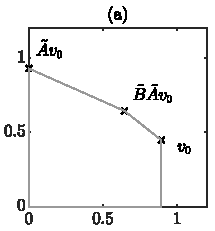
\includegraphics{./graphics/invpoly_1}
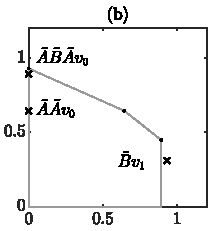
\includegraphics{./graphics/invpoly_2}
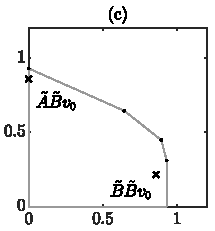
\includegraphics{./graphics/invpoly_3}
\end{center}

{\small%
\begin{lstlisting}
FIGURE(); hold on;
AE=[0 1.2 0 1.2]; TE=[0 .5 1]; %Axis and Ticks
A=[0 0;1 1]; B=[1 1;0 1]; cA={A,B}; 
tjsr(cA,'plot','polytope','fastnorm',0,'ordering',{[2 1 1]'});
Pi=B*B*A; rhoc=rho(Pi)^(1/3); At=A/rhoc; Bt=B/rhoc; Pit=Pi/rhoc^3; v1=1/sqrt(5)*[2;1];
V=[v1 At*v1 Bt*At*v1];
plotm(V,'x','Color',BLACK,'MarkerSize',DOTSIZE);
plotm(([V [0;0] [max(V(1,:));0] [0;max(V(2,:))]]),'hull','-','Color',LGREY,'LineWidth',LINESIZE);
TEXT(1,.4,'$v_0$');
TEXT(0.05,1.05,'$\tilde{A}v_0$'); 
TEXT(.7,.75,'$\tilde{B}\tilde{A}v_0$'); %cyclic root
SIZE(1,1); AXISE(AE); TICKS(TE,TE); LABEL('',''); TITLE('(a)'); POST();
SAVE('.','invpoly_1',EXT);
FIGURE(); hold on;
%V=V;
Vnew=[Bt*v1 At*At*v1 At*Bt*At*v1];
plotm(([V [0;0] [max(V(1,:));0] [0;max(V(2,:))]]),'hull','-','Color',LGREY,'LineWidth',LINESIZE);
plotm(V,'.','Color',BLACK,'MarkerSize',DOTSIZE);
plotm(Vnew,'x','Color',BLACK,'MarkerSize',DOTSIZE);
TEXT(.6,.3,'$\tilde{B}v_1$'); TEXT(.05,.65,'$\tilde{A}\tilde{A}v_0$'); TEXT(.05,1,'$\tilde{A}\tilde{B}\tilde{A}v_0$'); %new vertices
SIZE(1,1); AXISE(AE); TICKS(TE,TE); LABEL('',''); TITLE('(b)'); POST();
SAVE('.','invpoly_2',EXT);
FIGURE(); hold on;
V=[V Bt*v1]; 
Vnew=[Bt*Bt*v1 At*Bt*v1];
plotm(([V [0;0] [max(V(1,:));0] [0;max(V(2,:))]]),'hull','-','Color',LGREY,'LineWidth',LINESIZE);
plotm(V ,'.','Color',BLACK,'MarkerSize',DOTSIZE);
plotm(Vnew,'x','Color',BLACK,'MarkerSize',DOTSIZE);
TEXT(.55,.1,'$\tilde{B}\tilde{B}v_0$'); TEXT(.05,.7,'$\tilde{A}\tilde{B}v_0$'); %new vertices
SIZE(1,1); AXISE(AE); TICKS(TE,TE); LABEL('',''); TITLE('(c)'); POST();
SAVE('.','invpoly_3',EXT);
\end{lstlisting}%
}

\newpage
\section{Example 4.3}
\begin{center}
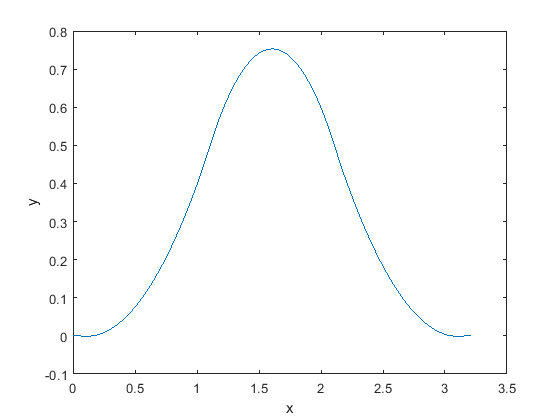
\includegraphics{./graphics/blf}	
\end{center}
\begin{lstlisting}
S = getS( 'a',sym(1/12)*[3 3 4 3 3 4 3 3 4 3 3].', 'M',-3, 'D',[-2 -1 0] )
[T,Om] = transitionmatrix( S )
V = constructVt( Om, 0 )
TV = restrictmatrix( T, V )
vdisp( -12.*TV )

tjsr( TV ); %with balancing
tjsr( TV, 'nobalancing' );

%%%%%%%%%%

FIGURE();
S=getS({1/12*[3 3 4 3 3 4 3 3 4 3 3]',-3,[]});
blf(S,'plot',{'Color',DGREY,'LineWidth',1}); 
SIZE(1.5,1); AXIS([-4 2 0 .3]); TICKS([-4 -2 0 2 4],[0 0.1 0.2 0.3]); LABEL('',''); POST();
SAVE('.','blf',EXT);
\end{lstlisting}


\section{Example 4.4}
{\small%
\begin{lstlisting}
E1 = [2 1;-1 2];
E2 = [2 0; 2 1];
tjsr( {E1,E2}, 'ordering',{[1 2]' [2 0]'}, 'smpflag',[0 1], ...
   'balancingvector',[1 0.95], 'invariantsubspace','none' )
\end{lstlisting}%
}

\section{Table 1 / Table 2}
The results are obtained with scripts similar to
{\small%
\begin{lstlisting}
dim = 10;
T = [];
i = 0;
while( i<10);
    M = tgallery( 'rand_gauss', dim, 2, 'norm' );
    [r,info] = tjsr( M );
    if( numel(r)==1 && info.info.errorcode<0 );
        i = i+1; 
        T(end+1) = info.counter.treetime; end;  end;
mean(T)
\end{lstlisting}%
}


\section{Table 3}
The results are obtained with scripts similar to
{\small%
\begin{lstlisting}
dim = 2;
J = 4;
i = 0;
[GRIP,MODGRIP] = deal( [] );
while( i<3 );
    M = tgallery( 'rand_gauss', dim, J, 'rho' );
    [r,info] = tjsr( M );
    if( numel(r)~=1 || info.info.errorcode>=0 );
        fprintf( ' Modified Invariant polytope algorithm did not find s.m.p..\n' );
        continue; end;
    i=i+1;
    
    [~,~,val] = findsmpold( M, 'gripenberg' );
    if( abs(val.jsrbound(1)-r)<1e-12 )
        GRIP(end+1) = val.time;
    else
        GRIP(end+1) = inf; end;
    
    [~,~,val] = findsmpold( M );
    if( abs(val.jsrbound(1)-r)<1e-12 )
        MODGRIP(end+1) = val.time;
    else
        MODGRIP(end+1) = false; end; end;
\end{lstlisting}%
}

\section{Example 5.1 / Table 4 / Table 5}
The results are obtained with scripts similar to
{\small%
\begin{lstlisting}
X = tgallery('mejstrik_119');
cmodgrip = findsmpold( X, 'maxsmpdepth',120 )
cgrip = findsmpold( X, 'gripenberg', 'delta',1, 'maxsmpdepth',120, 'v',2 )
cgen = findsmpold( X, 'genetic' )

C15 = tgallery('mejstrik_Cn',15)
cmodgrip = findsmpold( C15, 'maxsmpdepth',20 )
\end{lstlisting}%
}

\section{Table 6 / Table 7}
The results are obtained with scripts similar to
{\small%
\begin{lstlisting}
D = {[1 1],[1 -1],[-1 1],[-1 -1]};
C = codecapacity( D );
tjsr( C, 'v',2, 'maxsmpdepth',2 )
\end{lstlisting}%
}

\section{Table 8 / Figure 5}
\begin{center}
    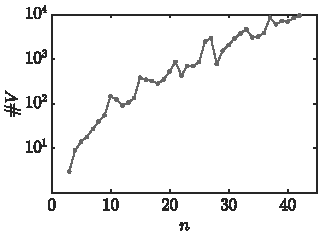
\includegraphics{./graphics/nVdaub}$\qquad$
    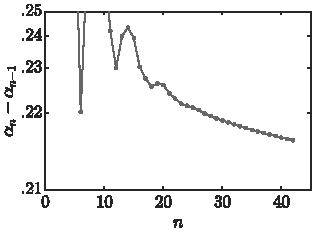
\includegraphics{./graphics/aldaub}
\end{center}
The figure is printed using
{\small%
\begin{lstlisting}
FIGURE(); 
V=[0 3 9 14 18 27 40 55 147 123 91 105 134 386 346 324 282 346 529 868 433 707 701 861 2471 2952 777 1545 2078 2898 3791 4692 3047 3191 3887 8529 6035 7142 6909 8343 9508];
n=[2 3 4 5 6 7 8 9 10 11 12 13 14 15 16 17 18 19 20 21 22 23 24 25 26 27 28 29 30 31 32 33 34 35 36 37 38 39 40 41 42];
semilogy(n,V,'o-','Color',DGREY,'MarkerSize',1,'MarkerFaceColor',DGREY);
set(findall(gcf,'-property','YMinorTick'),'YMinorTick','off')
SIZE(1.5,1); AXIS([0 45 1 10^4]); TICKS([0 10 20 30 40],[1e1 1e2 1e3 1e4]); LABEL('$n$','$\#V$'); TITLE(''); POST();
SAVE('.','nVdaub',EXT);

FIGURE();
n=[2 3 4 5 6 7 8 9 10 11 12 13 14 15 16 17 18 19 20 21 22 23 24 25 26 27 28 29 30 31 32 33 34 35 36 37 38 39 40 41 42];
al=[0.55001 1.08783 1.61793 1.96896 2.18914 2.46041 2.76082 3.07361 3.36139 3.60347 3.83348 4.07348 4.31676 4.55612 4.78644 5.01380 5.23917 5.46532 5.69108 5.91500 6.13779 6.35958 6.58096 6.80198 7.02250 7.24241 7.46187 7.68091 7.89962 8.11801 8.33605 8.55379 8.77123 8.98841 9.20533 9.42202 9.63847 9.85474 10.07073 10.28656 10.50220];
diffal=diff([0 al]);
semilogy(n,diffal-.2,'o-','Color',DGREY,'MarkerSize',1,'MarkerFaceColor',DGREY)
SIZE(1.5,1); AXIS([0 45 .01 .05]); TICKS([0 10 20 30 40],[0.01 .02 .03 .04 .05]); LABEL('$n$','$\alpha_n-\alpha_{n-1}$'); TICKLABELS({'0', '10', '20', '30', '40'},{'.21','.22','.23','.24','.25'});
SAVE('.','aldaub',EXT);
\end{lstlisting}%
}

The results from the table are obtained with scripts similar to
{\small%
\begin{lstlisting}
A = daubechiesmatrix( 10 );
tjsr( A, 'v',2 )
\end{lstlisting}%
}